% Options for packages loaded elsewhere
\PassOptionsToPackage{unicode}{hyperref}
\PassOptionsToPackage{hyphens}{url}
\PassOptionsToPackage{dvipsnames,svgnames,x11names}{xcolor}
%
\documentclass[
  ignorenonframetext,
]{beamer}
\usepackage{pgfpages}
\setbeamertemplate{caption}[numbered]
\setbeamertemplate{caption label separator}{: }
\setbeamercolor{caption name}{fg=normal text.fg}
\beamertemplatenavigationsymbolsempty
% Prevent slide breaks in the middle of a paragraph
\widowpenalties 1 10000
\raggedbottom
\setbeamertemplate{part page}{
  \centering
  \begin{beamercolorbox}[sep=16pt,center]{part title}
    \usebeamerfont{part title}\insertpart\par
  \end{beamercolorbox}
}
\setbeamertemplate{section page}{
  \centering
  \begin{beamercolorbox}[sep=12pt,center]{part title}
    \usebeamerfont{section title}\insertsection\par
  \end{beamercolorbox}
}
\setbeamertemplate{subsection page}{
  \centering
  \begin{beamercolorbox}[sep=8pt,center]{part title}
    \usebeamerfont{subsection title}\insertsubsection\par
  \end{beamercolorbox}
}
\AtBeginPart{
  \frame{\partpage}
}
\AtBeginSection{
  \ifbibliography
  \else
    \frame{\sectionpage}
  \fi
}
\AtBeginSubsection{
  \frame{\subsectionpage}
}
\usepackage{amsmath,amssymb}
\usepackage{lmodern}
\usepackage{iftex}
\ifPDFTeX
  \usepackage[T1]{fontenc}
  \usepackage[utf8]{inputenc}
  \usepackage{textcomp} % provide euro and other symbols
\else % if luatex or xetex
  \usepackage{unicode-math}
  \defaultfontfeatures{Scale=MatchLowercase}
  \defaultfontfeatures[\rmfamily]{Ligatures=TeX,Scale=1}
\fi
% Use upquote if available, for straight quotes in verbatim environments
\IfFileExists{upquote.sty}{\usepackage{upquote}}{}
\IfFileExists{microtype.sty}{% use microtype if available
  \usepackage[]{microtype}
  \UseMicrotypeSet[protrusion]{basicmath} % disable protrusion for tt fonts
}{}
\makeatletter
\@ifundefined{KOMAClassName}{% if non-KOMA class
  \IfFileExists{parskip.sty}{%
    \usepackage{parskip}
  }{% else
    \setlength{\parindent}{0pt}
    \setlength{\parskip}{6pt plus 2pt minus 1pt}}
}{% if KOMA class
  \KOMAoptions{parskip=half}}
\makeatother
\usepackage{xcolor}
\newif\ifbibliography
\usepackage{color}
\usepackage{fancyvrb}
\newcommand{\VerbBar}{|}
\newcommand{\VERB}{\Verb[commandchars=\\\{\}]}
\DefineVerbatimEnvironment{Highlighting}{Verbatim}{commandchars=\\\{\}}
% Add ',fontsize=\small' for more characters per line
\usepackage{framed}
\definecolor{shadecolor}{RGB}{248,248,248}
\newenvironment{Shaded}{\begin{snugshade}}{\end{snugshade}}
\newcommand{\AlertTok}[1]{\textcolor[rgb]{0.94,0.16,0.16}{#1}}
\newcommand{\AnnotationTok}[1]{\textcolor[rgb]{0.56,0.35,0.01}{\textbf{\textit{#1}}}}
\newcommand{\AttributeTok}[1]{\textcolor[rgb]{0.77,0.63,0.00}{#1}}
\newcommand{\BaseNTok}[1]{\textcolor[rgb]{0.00,0.00,0.81}{#1}}
\newcommand{\BuiltInTok}[1]{#1}
\newcommand{\CharTok}[1]{\textcolor[rgb]{0.31,0.60,0.02}{#1}}
\newcommand{\CommentTok}[1]{\textcolor[rgb]{0.56,0.35,0.01}{\textit{#1}}}
\newcommand{\CommentVarTok}[1]{\textcolor[rgb]{0.56,0.35,0.01}{\textbf{\textit{#1}}}}
\newcommand{\ConstantTok}[1]{\textcolor[rgb]{0.00,0.00,0.00}{#1}}
\newcommand{\ControlFlowTok}[1]{\textcolor[rgb]{0.13,0.29,0.53}{\textbf{#1}}}
\newcommand{\DataTypeTok}[1]{\textcolor[rgb]{0.13,0.29,0.53}{#1}}
\newcommand{\DecValTok}[1]{\textcolor[rgb]{0.00,0.00,0.81}{#1}}
\newcommand{\DocumentationTok}[1]{\textcolor[rgb]{0.56,0.35,0.01}{\textbf{\textit{#1}}}}
\newcommand{\ErrorTok}[1]{\textcolor[rgb]{0.64,0.00,0.00}{\textbf{#1}}}
\newcommand{\ExtensionTok}[1]{#1}
\newcommand{\FloatTok}[1]{\textcolor[rgb]{0.00,0.00,0.81}{#1}}
\newcommand{\FunctionTok}[1]{\textcolor[rgb]{0.00,0.00,0.00}{#1}}
\newcommand{\ImportTok}[1]{#1}
\newcommand{\InformationTok}[1]{\textcolor[rgb]{0.56,0.35,0.01}{\textbf{\textit{#1}}}}
\newcommand{\KeywordTok}[1]{\textcolor[rgb]{0.13,0.29,0.53}{\textbf{#1}}}
\newcommand{\NormalTok}[1]{#1}
\newcommand{\OperatorTok}[1]{\textcolor[rgb]{0.81,0.36,0.00}{\textbf{#1}}}
\newcommand{\OtherTok}[1]{\textcolor[rgb]{0.56,0.35,0.01}{#1}}
\newcommand{\PreprocessorTok}[1]{\textcolor[rgb]{0.56,0.35,0.01}{\textit{#1}}}
\newcommand{\RegionMarkerTok}[1]{#1}
\newcommand{\SpecialCharTok}[1]{\textcolor[rgb]{0.00,0.00,0.00}{#1}}
\newcommand{\SpecialStringTok}[1]{\textcolor[rgb]{0.31,0.60,0.02}{#1}}
\newcommand{\StringTok}[1]{\textcolor[rgb]{0.31,0.60,0.02}{#1}}
\newcommand{\VariableTok}[1]{\textcolor[rgb]{0.00,0.00,0.00}{#1}}
\newcommand{\VerbatimStringTok}[1]{\textcolor[rgb]{0.31,0.60,0.02}{#1}}
\newcommand{\WarningTok}[1]{\textcolor[rgb]{0.56,0.35,0.01}{\textbf{\textit{#1}}}}
\usepackage{graphicx}
\makeatletter
\def\maxwidth{\ifdim\Gin@nat@width>\linewidth\linewidth\else\Gin@nat@width\fi}
\def\maxheight{\ifdim\Gin@nat@height>\textheight\textheight\else\Gin@nat@height\fi}
\makeatother
% Scale images if necessary, so that they will not overflow the page
% margins by default, and it is still possible to overwrite the defaults
% using explicit options in \includegraphics[width, height, ...]{}
\setkeys{Gin}{width=\maxwidth,height=\maxheight,keepaspectratio}
% Set default figure placement to htbp
\makeatletter
\def\fps@figure{htbp}
\makeatother
\setlength{\emergencystretch}{3em} % prevent overfull lines
\providecommand{\tightlist}{%
  \setlength{\itemsep}{0pt}\setlength{\parskip}{0pt}}
\setcounter{secnumdepth}{-\maxdimen} % remove section numbering
\usepackage{graphicx}
\usepackage{bm}
\definecolor{foreground}{RGB}{255,255,255}
\definecolor{background}{RGB}{34,28,54}
\definecolor{title}{RGB}{105,165,255}
\definecolor{gray}{RGB}{175,175,175}
\definecolor{lightgray}{RGB}{225,225,225}
\definecolor{subtitle}{RGB}{232,234,255}
\definecolor{hilight}{RGB}{112,224,255}
\definecolor{vhilight}{RGB}{255,111,207}
\setbeamertemplate{footline}[page number]
\ifLuaTeX
  \usepackage{selnolig}  % disable illegal ligatures
\fi
\IfFileExists{bookmark.sty}{\usepackage{bookmark}}{\usepackage{hyperref}}
\IfFileExists{xurl.sty}{\usepackage{xurl}}{} % add URL line breaks if available
\urlstyle{same} % disable monospaced font for URLs
\hypersetup{
  pdftitle={STAT 528 - Advanced Regression Analysis II},
  pdfauthor={GLMM and GEE},
  colorlinks=true,
  linkcolor={Maroon},
  filecolor={Maroon},
  citecolor={Blue},
  urlcolor={blue},
  pdfcreator={LaTeX via pandoc}}

\title{STAT 528 - Advanced Regression Analysis II}
\author{GLMM and GEE}
\date{}
\institute{Daniel J. Eck\\
Department of Statistics\\
University of Illinois}

\begin{document}
\frame{\titlepage}

\begin{frame}
\newcommand{\R}{\mathbb{R}}
\end{frame}

\begin{frame}{Learning Objectives Today}
\protect\hypertarget{learning-objectives-today}{}
\begin{itemize}
\tightlist
\item
  GLMM examples
\item
  GEE theory
\item
  GEE examples
\end{itemize}
\end{frame}

\begin{frame}[fragile]{}
\protect\hypertarget{section}{}
We load in necessary packages.

\vspace{12pt}

\begin{Shaded}
\begin{Highlighting}[]
\FunctionTok{library}\NormalTok{(faraway)}
\FunctionTok{library}\NormalTok{(tidyverse)}
\FunctionTok{library}\NormalTok{(ggplot2)}
\FunctionTok{library}\NormalTok{(MASS)}
\FunctionTok{library}\NormalTok{(lme4)}
\FunctionTok{library}\NormalTok{(INLA)}
\FunctionTok{library}\NormalTok{(glmm)}
\FunctionTok{library}\NormalTok{(parallel)}
\end{Highlighting}
\end{Shaded}
\end{frame}

\begin{frame}[fragile]{}
\protect\hypertarget{section-1}{}
In this example, we have data from a clinical trial of 59 epileptics.

For a baseline, patients were observed for 8 weeks and the number of
seizures recorded. The patients were then randomized to treatment by the
drug Progabide (31 patients) or to the placebo group (28 patients).

They were observed for four 2-week periods and the number of seizures
recorded. We are interested in determining whether Progabide reduces the
rate of seizures.

We first perform some data manipulations and then look at the first few
observations:

\vspace{12pt}
\tiny

\begin{Shaded}
\begin{Highlighting}[]
\FunctionTok{data}\NormalTok{(epilepsy, }\AttributeTok{package=}\StringTok{"faraway"}\NormalTok{)}
\NormalTok{epilepsy}\SpecialCharTok{$}\NormalTok{period }\OtherTok{\textless{}{-}} \FunctionTok{rep}\NormalTok{(}\DecValTok{0}\SpecialCharTok{:}\DecValTok{4}\NormalTok{, }\DecValTok{59}\NormalTok{)}
\NormalTok{epilepsy}\SpecialCharTok{$}\NormalTok{drug }\OtherTok{\textless{}{-}} \FunctionTok{factor}\NormalTok{(}\FunctionTok{c}\NormalTok{(}\StringTok{"placebo"}\NormalTok{,}\StringTok{"treatment"}\NormalTok{)[epilepsy}\SpecialCharTok{$}\NormalTok{treat}\SpecialCharTok{+}\DecValTok{1}\NormalTok{])}
\NormalTok{epilepsy}\SpecialCharTok{$}\NormalTok{phase }\OtherTok{\textless{}{-}} \FunctionTok{factor}\NormalTok{(}\FunctionTok{c}\NormalTok{(}\StringTok{"baseline"}\NormalTok{,}\StringTok{"experiment"}\NormalTok{)[epilepsy}\SpecialCharTok{$}\NormalTok{expind }\SpecialCharTok{+}\DecValTok{1}\NormalTok{])}
\NormalTok{epilepsy }\SpecialCharTok{\%\textgreater{}\%} \FunctionTok{filter}\NormalTok{(id }\SpecialCharTok{\textless{}} \FloatTok{2.5}\NormalTok{) }\SpecialCharTok{\%\textgreater{}\%} \FunctionTok{head}\NormalTok{(}\DecValTok{3}\NormalTok{)}
\end{Highlighting}
\end{Shaded}

\begin{verbatim}
##   seizures id treat expind timeadj age period    drug      phase
## 1       11  1     0      0       8  31      0 placebo   baseline
## 2        5  1     0      1       2  31      1 placebo experiment
## 3        3  1     0      1       2  31      2 placebo experiment
\end{verbatim}
\end{frame}

\begin{frame}[fragile]{}
\protect\hypertarget{section-2}{}
The variables are:

\begin{itemize}
\tightlist
\item
  \texttt{expind} indicates the baseline phase by 0 and the treatment
  phase by 1.\\
\item
  \texttt{timeadj} indicates the time phases.
\end{itemize}

Three new convenience variables are created:

\begin{itemize}
\tightlist
\item
  \texttt{period} denotes the separate 2- or 8- week periods
\item
  \texttt{drug} records the type of treatment in nonnumeric form
\item
  \texttt{phase} indicates the phase of the experiment
\end{itemize}

We now compute the mean number of seizures per week broken down by the
treatment and baseline vs.~experimental period.

\vspace{12pt}
\tiny

\begin{Shaded}
\begin{Highlighting}[]
\NormalTok{epilepsy }\SpecialCharTok{\%\textgreater{}\%} 
  \FunctionTok{group\_by}\NormalTok{(drug, phase) }\SpecialCharTok{\%\textgreater{}\%} 
  \FunctionTok{summarise}\NormalTok{(}\AttributeTok{rate=}\FunctionTok{mean}\NormalTok{(seizures}\SpecialCharTok{/}\NormalTok{timeadj)) }\SpecialCharTok{\%\textgreater{}\%}
\FunctionTok{xtabs}\NormalTok{(}\AttributeTok{formula=}\NormalTok{rate }\SpecialCharTok{\textasciitilde{}}\NormalTok{ phase }\SpecialCharTok{+}\NormalTok{ drug)}
\end{Highlighting}
\end{Shaded}

\begin{verbatim}
##             drug
## phase         placebo treatment
##   baseline   3.848214  3.955645
##   experiment 4.303571  3.983871
\end{verbatim}
\end{frame}

\begin{frame}{}
\protect\hypertarget{section-3}{}
We see that the rate of seizures in the treatment group actually
increases during the period in which the drug was taken. The rate of
seizures increases even more in the placebo group.

Perhaps some other factor is causing the rate of seizures to increase
during the treatment period and the drug is actually having a beneficial
effect.

Now we make some plots to show the difference between the treatment and
the control. The first plot shows the difference between the two groups
during the experimental period only:
\end{frame}

\begin{frame}{}
\protect\hypertarget{section-4}{}
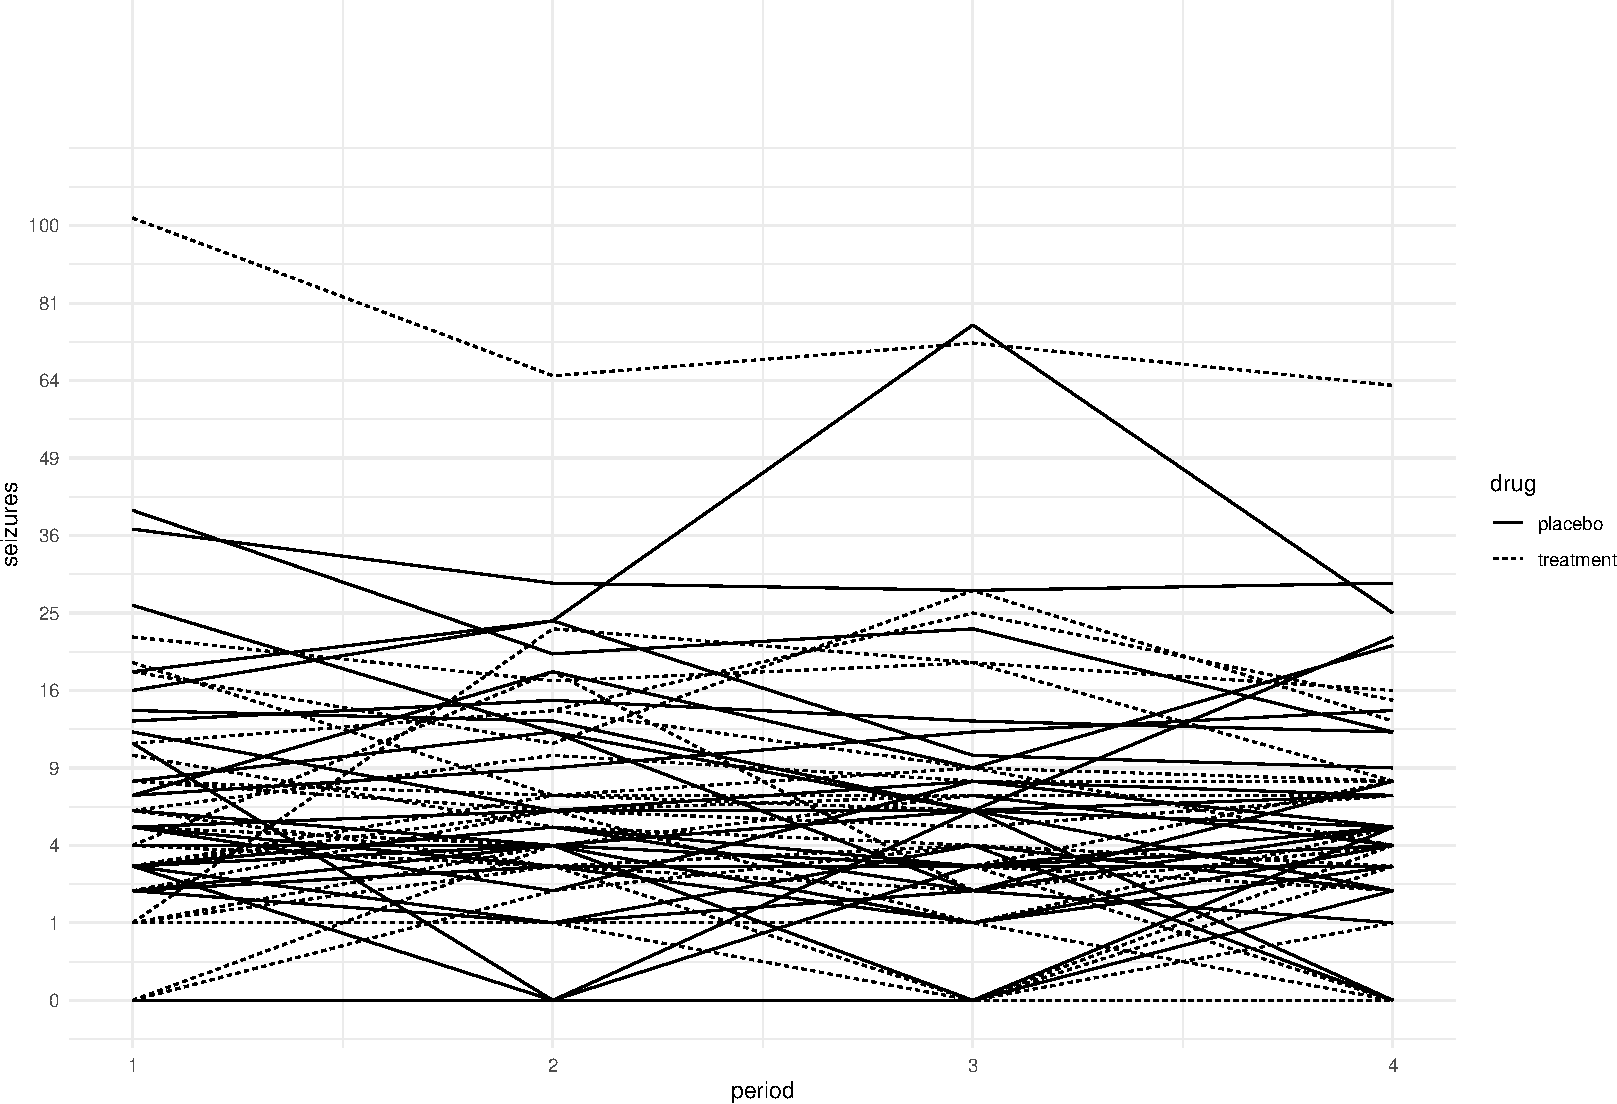
\includegraphics{week13p2_files/figure-beamer/unnamed-chunk-4-1.pdf}
\end{frame}

\begin{frame}{}
\protect\hypertarget{section-5}{}
We now compare the average seizure rate to the baseline for the two
groups. The square-root transform is used to stabilize the variance;
this is often used with count data.

\vspace{12pt}

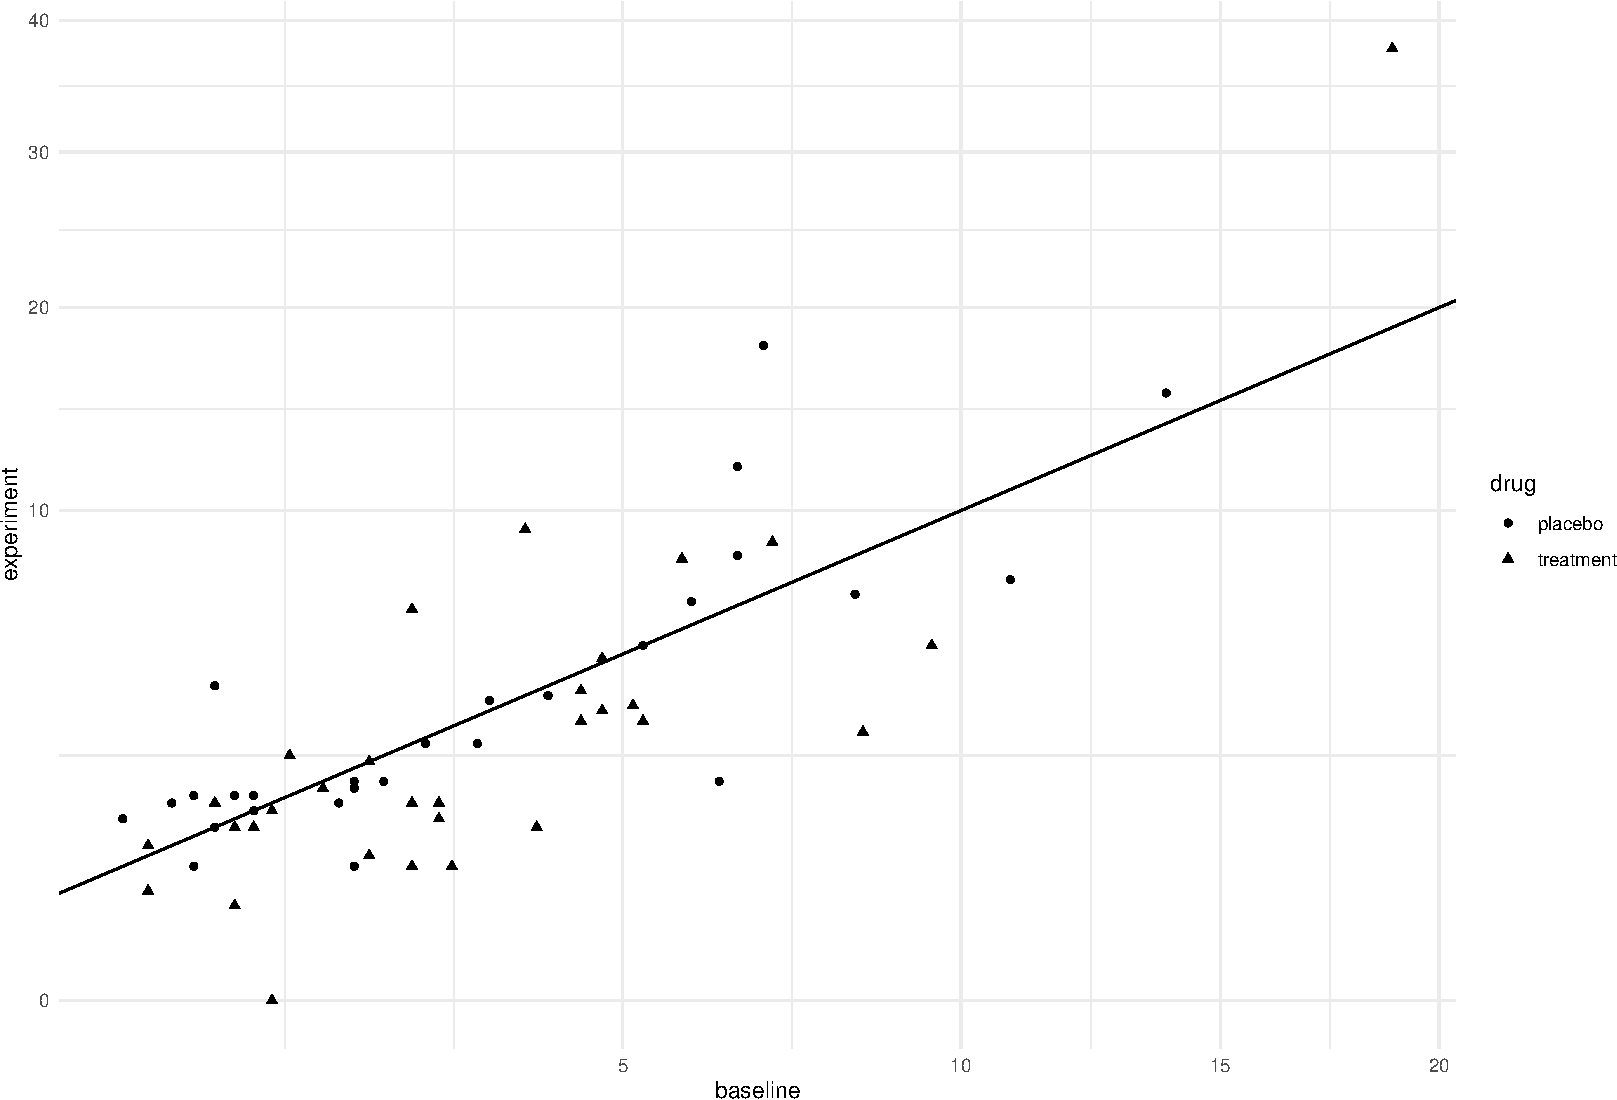
\includegraphics{week13p2_files/figure-beamer/unnamed-chunk-5-1.pdf}
\end{frame}

\begin{frame}[fragile]{}
\protect\hypertarget{section-6}{}
A treatment effect, if one exists, is not readily apparent. Now we fit
GLMM models. Patient \#49 is unusual because of the high rate of
seizures observed. We exclude it:

\vspace{12pt}
\small

\begin{Shaded}
\begin{Highlighting}[]
\NormalTok{epilo }\OtherTok{\textless{}{-}} \FunctionTok{filter}\NormalTok{(epilepsy, id }\SpecialCharTok{!=} \DecValTok{49}\NormalTok{)}
\end{Highlighting}
\end{Shaded}

\vspace{12pt}
\normalsize

Excluding a case should not be taken lightly. For projects where the
analyst works with producers of the data, it will be possible to discuss
substantive reasons for excluding cases.

It is worth starting with a GLM even though the model is not correct due
to the grouping of the observations. We must use an offset to allow for
the difference in lengths in the baseline and treatment periods:

\[
\log\frac{\mu_i}{t_i} = x_i^T\beta
\]
\end{frame}

\begin{frame}[fragile]{}
\protect\hypertarget{section-7}{}
\tiny

\begin{Shaded}
\begin{Highlighting}[]
\NormalTok{modglm }\OtherTok{\textless{}{-}} \FunctionTok{glm}\NormalTok{(seizures }\SpecialCharTok{\textasciitilde{}}\FunctionTok{offset}\NormalTok{(}\FunctionTok{log}\NormalTok{(timeadj)) }\SpecialCharTok{+}\NormalTok{ expind }\SpecialCharTok{+}\NormalTok{ treat }\SpecialCharTok{+} 
  \FunctionTok{I}\NormalTok{(expind}\SpecialCharTok{*}\NormalTok{treat), }\AttributeTok{family=}\NormalTok{poisson, }\AttributeTok{data=}\NormalTok{epilo)}
\FunctionTok{summary}\NormalTok{(modglm)}
\end{Highlighting}
\end{Shaded}

\begin{verbatim}
## 
## Call:
## glm(formula = seizures ~ offset(log(timeadj)) + expind + treat + 
##     I(expind * treat), family = poisson, data = epilo)
## 
## Deviance Residuals: 
##     Min       1Q   Median       3Q      Max  
## -5.4725  -2.3605  -1.0290   0.9001  14.0104  
## 
## Coefficients:
##                   Estimate Std. Error z value Pr(>|z|)    
## (Intercept)        1.34761    0.03406  39.566  < 2e-16 ***
## expind             0.11184    0.04688   2.386    0.017 *  
## treat             -0.10682    0.04863  -2.197    0.028 *  
## I(expind * treat) -0.30238    0.06971  -4.338 1.44e-05 ***
## ---
## Signif. codes:  0 '***' 0.001 '**' 0.01 '*' 0.05 '.' 0.1 ' ' 1
## 
## (Dispersion parameter for poisson family taken to be 1)
## 
##     Null deviance: 2485.1  on 289  degrees of freedom
## Residual deviance: 2411.5  on 286  degrees of freedom
## AIC: 3449.7
## 
## Number of Fisher Scoring iterations: 5
\end{verbatim}
\end{frame}

\begin{frame}{}
\protect\hypertarget{section-8}{}
The interaction term is the primary parameter of interest. All the
subjects were untreated in the baseline. This means that the main effect
for treatment does not properly measure the response to treatment
because it includes the baseline period.

As we have observed already, we suspect the response may have been
different during the baseline time and the active period of the
experiment. The interaction term represents the effect of the treatment
during the baseline period after adjustment. In the output above we see
that this interaction seems highly significant and negative (which is
good since we want to reduce seizures).

But this inference is suspect because we have made no allowance for the
correlated responses within individuals. The p-value is far smaller than
it should be.
\end{frame}

\begin{frame}[fragile]{PQL methods}
\protect\hypertarget{pql-methods}{}
\tiny

\begin{Shaded}
\begin{Highlighting}[]
\NormalTok{modpql }\OtherTok{\textless{}{-}} \FunctionTok{glmmPQL}\NormalTok{(seizures }\SpecialCharTok{\textasciitilde{}}\FunctionTok{offset}\NormalTok{(}\FunctionTok{log}\NormalTok{(timeadj)) }\SpecialCharTok{+}\NormalTok{ expind }\SpecialCharTok{+}\NormalTok{ treat }\SpecialCharTok{+} 
  \FunctionTok{I}\NormalTok{(expind}\SpecialCharTok{*}\NormalTok{treat), }\AttributeTok{random =} \SpecialCharTok{\textasciitilde{}}\DecValTok{1}\SpecialCharTok{|}\NormalTok{id, }\AttributeTok{family=}\NormalTok{poisson, }\AttributeTok{data=}\NormalTok{epilo)}
\FunctionTok{summary}\NormalTok{(modpql)}
\end{Highlighting}
\end{Shaded}

\begin{verbatim}
## Linear mixed-effects model fit by maximum likelihood
##   Data: epilo 
##   AIC BIC logLik
##    NA  NA     NA
## 
## Random effects:
##  Formula: ~1 | id
##         (Intercept) Residual
## StdDev:   0.6820012 1.605385
## 
## Variance function:
##  Structure: fixed weights
##  Formula: ~invwt 
## Fixed effects:  seizures ~ offset(log(timeadj)) + expind + treat + I(expind *      treat) 
##                        Value  Std.Error  DF   t-value p-value
## (Intercept)        1.0761832 0.09990514 230 10.772050  0.0000
## expind             0.1125119 0.07412152 230  1.517939  0.1304
## I(expind * treat) -0.3037615 0.10819095 230 -2.807642  0.0054
##  Correlation: 
##                   (Intr) expind
## expind            -0.198       
## I(expind * treat) -0.014 -0.656
## 
## Standardized Within-Group Residuals:
##        Min         Q1        Med         Q3        Max 
## -2.2934834 -0.5649468 -0.1492931  0.3224895  6.3123337 
## 
## Number of Observations: 290
## Number of Groups: 58
\end{verbatim}
\end{frame}

\begin{frame}{}
\protect\hypertarget{section-9}{}
The parameter estimates from the PQL fit are comparable to the GLM fit.
However, the standard errors are larger in the PQL fit as might be
expected given that the correlated responses have been allowed for.

As with the binary response example, we still have some doubts about the
accuracy of the inference. This is a particular concern when some count
responses are small.
\end{frame}

\begin{frame}[fragile]{Numerical integration}
\protect\hypertarget{numerical-integration}{}
Numerical quadrature can also be used. We use Gauss-Hermite in
preference to Laplace as the model random effect structure is simple and
so the computation is fast even though we have used the most expensive
\texttt{nAGQ=25} setting. \vspace{12pt} \tiny

\begin{Shaded}
\begin{Highlighting}[]
\NormalTok{modgh }\OtherTok{\textless{}{-}} \FunctionTok{glmer}\NormalTok{(seizures }\SpecialCharTok{\textasciitilde{}}\FunctionTok{offset}\NormalTok{(}\FunctionTok{log}\NormalTok{(timeadj)) }\SpecialCharTok{+}\NormalTok{ expind }\SpecialCharTok{+}\NormalTok{ treat }\SpecialCharTok{+} 
  \FunctionTok{I}\NormalTok{(expind}\SpecialCharTok{*}\NormalTok{treat)}\SpecialCharTok{+}\NormalTok{ (}\DecValTok{1}\SpecialCharTok{|}\NormalTok{id), }\AttributeTok{nAGQ=}\DecValTok{25}\NormalTok{, }\AttributeTok{family=}\NormalTok{poisson, }\AttributeTok{data=}\NormalTok{epilo)}
\end{Highlighting}
\end{Shaded}
\end{frame}

\begin{frame}[fragile]{}
\protect\hypertarget{section-10}{}
\tiny

\begin{Shaded}
\begin{Highlighting}[]
\FunctionTok{summary}\NormalTok{(modgh)}
\end{Highlighting}
\end{Shaded}

\begin{verbatim}
## Generalized linear mixed model fit by maximum likelihood (Adaptive
##   Gauss-Hermite Quadrature, nAGQ = 25) [glmerMod]
##  Family: poisson  ( log )
## Formula: seizures ~ offset(log(timeadj)) + expind + treat + I(expind *  
##     treat) + (1 | id)
##    Data: epilo
## 
##      AIC      BIC   logLik deviance df.resid 
##    877.7    896.1   -433.9    867.7      285 
## 
## Scaled residuals: 
##     Min      1Q  Median      3Q     Max 
## -3.8724 -0.8482 -0.1722  0.5697  9.8941 
## 
## Random effects:
##  Groups Name        Variance Std.Dev.
##  id     (Intercept) 0.515    0.7176  
## Number of obs: 290, groups:  id, 58
## 
## Fixed effects:
##                    Estimate Std. Error z value Pr(>|z|)    
## (Intercept)        1.035998   0.141256   7.334 2.23e-13 ***
## expind             0.111838   0.046877   2.386    0.017 *  
## treat             -0.008152   0.196525  -0.041    0.967    
## I(expind * treat) -0.302387   0.069714  -4.338 1.44e-05 ***
## ---
## Signif. codes:  0 '***' 0.001 '**' 0.01 '*' 0.05 '.' 0.1 ' ' 1
## 
## Correlation of Fixed Effects:
##             (Intr) expind treat 
## expind      -0.175              
## treat       -0.718  0.126       
## I(xpnd*trt)  0.118 -0.672 -0.173
\end{verbatim}
\end{frame}

\begin{frame}[fragile]{}
\protect\hypertarget{section-11}{}
We see that the interaction effect is significant. Notice that the
estimate of this effect has been quite consistent over all the
estimation methods so we draw some confidence from this. We have

\vspace{12pt}

\begin{Shaded}
\begin{Highlighting}[]
\FunctionTok{exp}\NormalTok{(}\SpecialCharTok{{-}}\FloatTok{0.302}\NormalTok{)}
\end{Highlighting}
\end{Shaded}

\begin{verbatim}
## [1] 0.7393381
\end{verbatim}

\vspace{12pt}

So the drug is estimated to reduce the rate of seizures by about 26\%.
However, the subject SD is more than twice the drug effect of -0.3 at
0.718. This indicates that the expected improvement in the drug is
substantially less than the variation between individuals.
\end{frame}

\begin{frame}{}
\protect\hypertarget{section-12}{}
Interpretation of the main effect terms is problematic in the presence
of an interaction. For example, the treatment effect reported here
represents the predicted difference in the response during the baseline
period (i.e., \texttt{expind=0}).

Since none of the subjects are treated during the baseline period, we
are reassured to see that this effect is not significant.

However, this does illustrate the danger in naively presuming that this
is the treatment effect.
\end{frame}

\begin{frame}[fragile]{Bayesian methods}
\protect\hypertarget{bayesian-methods}{}
We can also take a Bayesian approach using \texttt{INLA}.

\vspace{12pt}
\tiny

\begin{Shaded}
\begin{Highlighting}[]
\NormalTok{formula }\OtherTok{\textless{}{-}}\NormalTok{ seizures }\SpecialCharTok{\textasciitilde{}} \FunctionTok{offset}\NormalTok{(}\FunctionTok{log}\NormalTok{(timeadj)) }\SpecialCharTok{+}\NormalTok{ expind }\SpecialCharTok{+}\NormalTok{ treat }\SpecialCharTok{+} 
  \FunctionTok{I}\NormalTok{(expind}\SpecialCharTok{*}\NormalTok{treat) }\SpecialCharTok{+} \FunctionTok{f}\NormalTok{(id,}\AttributeTok{model=}\StringTok{"iid"}\NormalTok{)}
\NormalTok{result }\OtherTok{\textless{}{-}} \FunctionTok{inla}\NormalTok{(formula, }\AttributeTok{family=}\StringTok{"poisson"}\NormalTok{, }\AttributeTok{data =}\NormalTok{ epilo)}
\end{Highlighting}
\end{Shaded}

\vspace{12pt}
\normalsize

We obtain a summary of the posteriors as:

\vspace{12pt}
\tiny

\begin{Shaded}
\begin{Highlighting}[]
\NormalTok{sigmaalpha }\OtherTok{\textless{}{-}} \FunctionTok{inla.tmarginal}\NormalTok{(}\ControlFlowTok{function}\NormalTok{(x) }\DecValTok{1}\SpecialCharTok{/}\FunctionTok{sqrt}\NormalTok{(x), }
\NormalTok{  result}\SpecialCharTok{$}\NormalTok{marginals.hyperpar}\SpecialCharTok{$}\StringTok{"Precision for id"}\NormalTok{)}
\NormalTok{restab }\OtherTok{\textless{}{-}} \FunctionTok{sapply}\NormalTok{(result}\SpecialCharTok{$}\NormalTok{marginals.fixed, }
  \ControlFlowTok{function}\NormalTok{(x) }\FunctionTok{inla.zmarginal}\NormalTok{(x, }\AttributeTok{silent=}\ConstantTok{TRUE}\NormalTok{))}
\NormalTok{restab }\OtherTok{\textless{}{-}} \FunctionTok{cbind}\NormalTok{(restab, }
  \FunctionTok{inla.zmarginal}\NormalTok{(sigmaalpha, }\AttributeTok{silent=}\ConstantTok{TRUE}\NormalTok{))}
\FunctionTok{colnames}\NormalTok{(restab) }\OtherTok{=} \FunctionTok{c}\NormalTok{(}\StringTok{"mu"}\NormalTok{,}\StringTok{"expind"}\NormalTok{,}\StringTok{"treat"}\NormalTok{,}
  \StringTok{"interaction"}\NormalTok{,}\StringTok{"alpha"}\NormalTok{)}
\FunctionTok{data.frame}\NormalTok{(restab)}
\end{Highlighting}
\end{Shaded}

\begin{verbatim}
##                   mu     expind        treat interaction      alpha
## mean        1.036115  0.1118965  -0.00825552  -0.3025702  0.7254792
## sd         0.1421983 0.04685179    0.1978247  0.06967626 0.07183047
## quant0.025 0.7550146 0.01995068   -0.3978168  -0.4393086    0.59977
## quant0.25  0.9410767 0.08018646    -0.140758  -0.3497282  0.6746726
## quant0.5    1.036183  0.1117989 -0.008691486  -0.3027154   0.719905
## quant0.75   1.130938  0.1434113     0.123375  -0.2557025  0.7702153
## quant0.975  1.314419  0.2036471     0.380427  -0.1661221  0.8818008
\end{verbatim}

\vspace{12pt}
\normalsize

We see that the results are similar to those obtained previously. We
observe that the 95\% credible interval for the interaction is
(-0.44,-0.17) so we are sure that this parameter differs from zero. We
compute similar plots as we did in the binary response example.
\end{frame}

\begin{frame}{}
\protect\hypertarget{section-13}{}
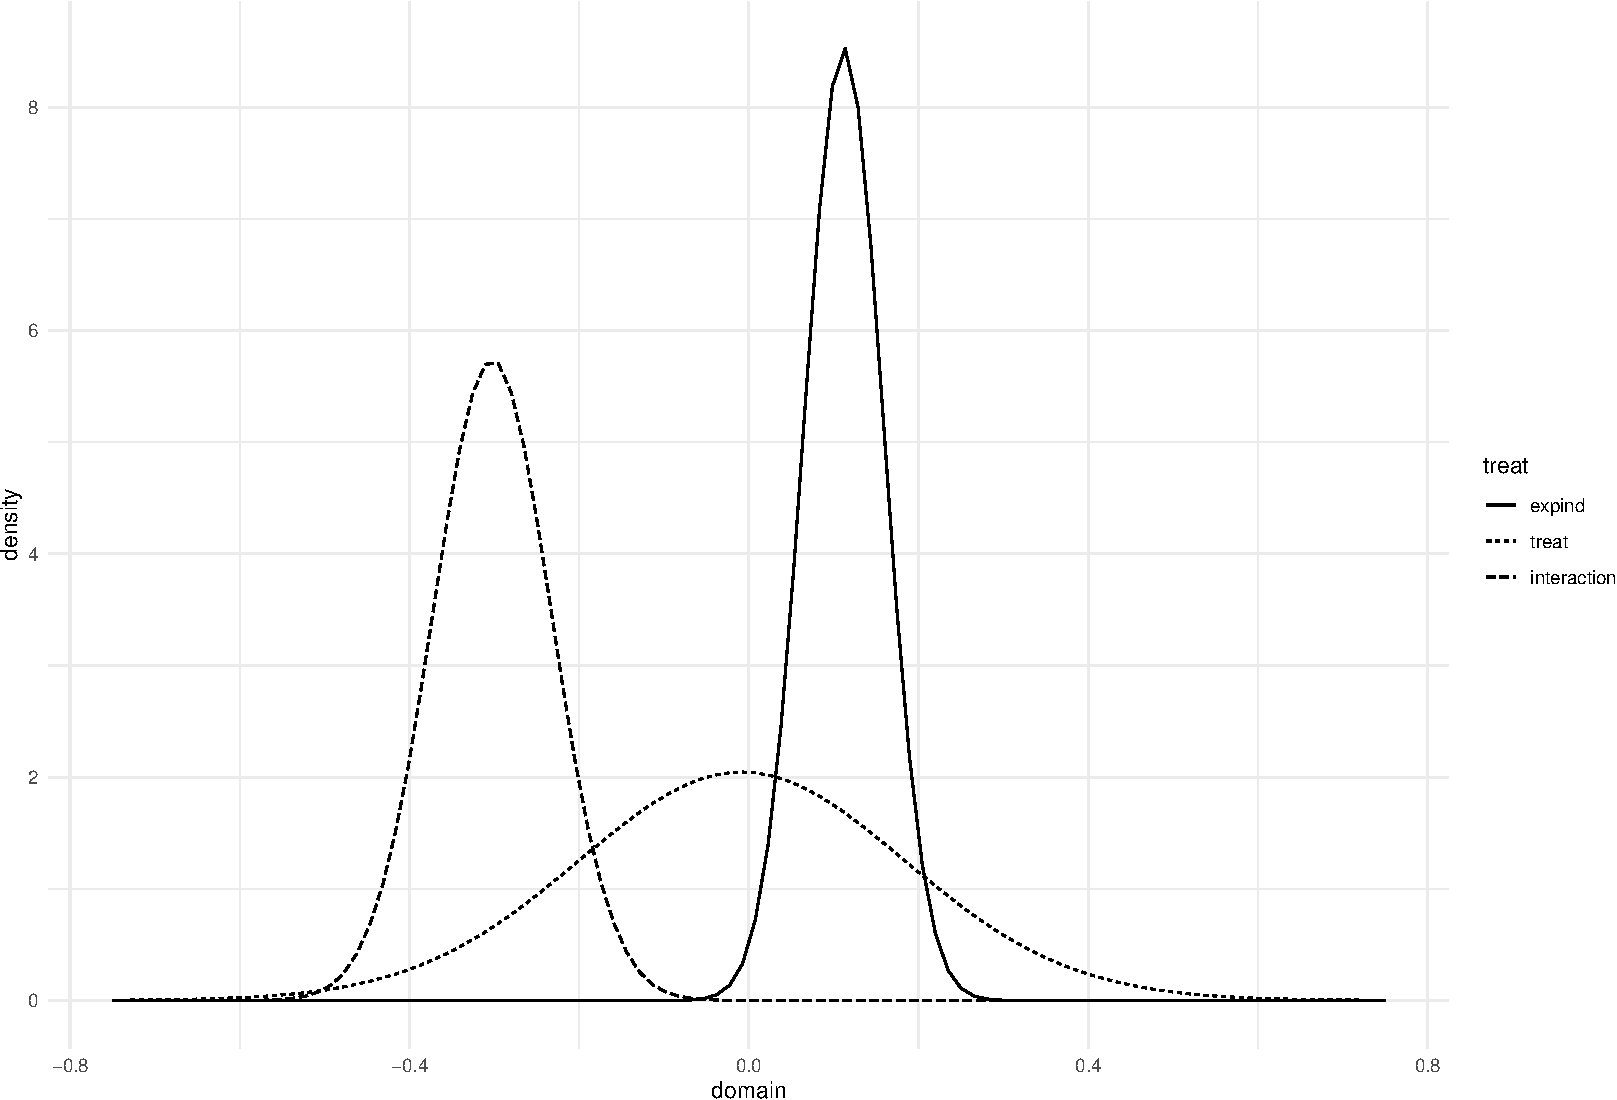
\includegraphics{week13p2_files/figure-beamer/unnamed-chunk-14-1.pdf}
\end{frame}

\begin{frame}[fragile]{Monte Carlo likelihood approximation}
\protect\hypertarget{monte-carlo-likelihood-approximation}{}
We can use the \texttt{glmm} package to implement the MCLA approach to
fitting GLMM models with Poisson responses.

\vspace{12pt}
\tiny

\begin{Shaded}
\begin{Highlighting}[]
\NormalTok{epilo}\SpecialCharTok{$}\NormalTok{idF }\OtherTok{\textless{}{-}} \FunctionTok{as.factor}\NormalTok{(epilo}\SpecialCharTok{$}\NormalTok{id)}
\NormalTok{epilo}\SpecialCharTok{$}\NormalTok{seizures }\OtherTok{\textless{}{-}} \FunctionTok{as.integer}\NormalTok{(epilo}\SpecialCharTok{$}\NormalTok{seizures)}
\FunctionTok{set.seed}\NormalTok{(}\DecValTok{13}\NormalTok{)}
\NormalTok{clust }\OtherTok{\textless{}{-}} \FunctionTok{makeCluster}\NormalTok{(}\DecValTok{8}\NormalTok{)}
\FunctionTok{system.time}\NormalTok{(m1 }\OtherTok{\textless{}{-}} \FunctionTok{glmm}\NormalTok{(seizures }\SpecialCharTok{\textasciitilde{}} \FunctionTok{offset}\NormalTok{(}\FunctionTok{log}\NormalTok{(timeadj)) }\SpecialCharTok{+} 
\NormalTok{  expind }\SpecialCharTok{+}\NormalTok{ treat }\SpecialCharTok{+} \FunctionTok{I}\NormalTok{(expind}\SpecialCharTok{*}\NormalTok{treat), }\AttributeTok{random =} \FunctionTok{list}\NormalTok{(}\SpecialCharTok{\textasciitilde{}}\DecValTok{0}\SpecialCharTok{+}\NormalTok{idF), }
  \AttributeTok{family.glmm =}\NormalTok{ poisson.glmm, }\AttributeTok{m =} \FloatTok{7e4}\NormalTok{, }
  \AttributeTok{varcomps.names =} \FunctionTok{c}\NormalTok{(}\StringTok{"idF"}\NormalTok{), }\AttributeTok{cluster =}\NormalTok{ clust, }\AttributeTok{data=}\NormalTok{epilo))}
\end{Highlighting}
\end{Shaded}

\begin{verbatim}
##    user  system elapsed 
##   6.095   0.653  66.986
\end{verbatim}
\end{frame}

\begin{frame}[fragile]{}
\protect\hypertarget{section-14}{}
We obtain summary information. However, the fit is buggy. The Monte
Carlo standard error is not returned and the summary table estimates are
not depicted.

\vspace{12pt}
\tiny

\begin{Shaded}
\begin{Highlighting}[]
\DocumentationTok{\#\# takes awhile to load}
\FunctionTok{summary}\NormalTok{(m1)}
\end{Highlighting}
\end{Shaded}

\begin{verbatim}
## 
## Call:
## glmm(fixed = seizures ~ offset(log(timeadj)) + expind + treat + 
##     I(expind * treat), random = list(~0 + idF), varcomps.names = c("idF"), 
##     data = epilo, family.glmm = poisson.glmm, m = 70000, cluster = clust)
## 
## 
## Link is: "log"
## 
## Fixed Effects:
##                   Estimate Std. Error z value Pr(>|z|)    
## (Intercept)              0          0  31.010  < 2e-16 ***
## expind                   0          0 -27.187  < 2e-16 ***
## treat                    0          0   0.018    0.986    
## I(expind * treat)        0          0  -4.338 1.44e-05 ***
## ---
## Signif. codes:  0 '***' 0.001 '**' 0.01 '*' 0.05 '.' 0.1 ' ' 1
## 
## 
## Variance Components for Random Effects (P-values are one-tailed):
##     Estimate Std. Error z value Pr(>|z|)/2    
## idF        0          0   5.098   1.72e-07 ***
## ---
## Signif. codes:  0 '***' 0.001 '**' 0.01 '*' 0.05 '.' 0.1 ' ' 1
\end{verbatim}
\end{frame}

\begin{frame}[fragile]{}
\protect\hypertarget{section-15}{}
\tiny

\begin{Shaded}
\begin{Highlighting}[]
\CommentTok{\# Monte Carlo standard errors}
\NormalTok{mcse\_glmm }\OtherTok{\textless{}{-}} \FunctionTok{mcse}\NormalTok{(m1)}
\NormalTok{mcse\_glmm}
\end{Highlighting}
\end{Shaded}

\begin{verbatim}
##       (Intercept)            expind             treat I(expind * treat) 
##               NaN               NaN               NaN               NaN 
##               idF 
##               NaN
\end{verbatim}
\end{frame}

\begin{frame}[fragile]{}
\protect\hypertarget{section-16}{}
That being said, we can obtain estimates of fixed effects and their
standard errors from objects in the \texttt{glmm} object.

\vspace{12pt}
\tiny

\begin{Shaded}
\begin{Highlighting}[]
\CommentTok{\# standard errors}
\NormalTok{se\_glmm }\OtherTok{\textless{}{-}} \FunctionTok{se}\NormalTok{(m1)}

\CommentTok{\# table for fixed effects}
\NormalTok{tab }\OtherTok{\textless{}{-}} \FunctionTok{cbind}\NormalTok{(m1}\SpecialCharTok{$}\NormalTok{beta, se\_glmm[}\SpecialCharTok{{-}}\DecValTok{5}\NormalTok{], m1}\SpecialCharTok{$}\NormalTok{beta}\SpecialCharTok{/}\NormalTok{se\_glmm[}\SpecialCharTok{{-}}\DecValTok{5}\NormalTok{])}
\FunctionTok{colnames}\NormalTok{(tab) }\OtherTok{\textless{}{-}} \FunctionTok{c}\NormalTok{(}\StringTok{"Estimate"}\NormalTok{, }\StringTok{"Std. Error"}\NormalTok{, }\StringTok{"z value"}\NormalTok{)}
\FunctionTok{round}\NormalTok{(tab, }\DecValTok{3}\NormalTok{)}
\end{Highlighting}
\end{Shaded}

\begin{verbatim}
##                   Estimate Std. Error z value
## (Intercept)          3.106      0.100  31.010
## expind              -1.274      0.047 -27.187
## treat                0.003      0.185   0.018
## I(expind * treat)   -0.302      0.070  -4.338
\end{verbatim}
\end{frame}

\begin{frame}[fragile]{}
\protect\hypertarget{section-17}{}
We can also obtain estimates of random effect parameters and their
standard errors from objects in the \texttt{glmm} object.

\vspace{12pt}
\tiny

\begin{Shaded}
\begin{Highlighting}[]
\FunctionTok{c}\NormalTok{(m1}\SpecialCharTok{$}\NormalTok{nu, se\_glmm[}\DecValTok{5}\NormalTok{])}
\end{Highlighting}
\end{Shaded}

\begin{verbatim}
##       idF       idF 
## 0.5152511 0.1010674
\end{verbatim}

\vspace{12pt}
\normalsize

Important parameter estimates are similar to the other fitting
techniques which instills some confidence.
\end{frame}

\begin{frame}{}
\protect\hypertarget{section-18}{}
\begin{center}
\Large Discuss GEE
\end{center}
\end{frame}

\begin{frame}[fragile]{}
\protect\hypertarget{section-19}{}
We will use the \texttt{geepack} package to fit GEEs. We will reanalyze
the stability dataset using generalized estimating equations.

\vspace{12pt}
\tiny

\begin{Shaded}
\begin{Highlighting}[]
\FunctionTok{library}\NormalTok{(geepack)}
\FunctionTok{data}\NormalTok{(ctsib)}
\NormalTok{ctsib}\SpecialCharTok{$}\NormalTok{stable }\OtherTok{\textless{}{-}} \FunctionTok{ifelse}\NormalTok{(ctsib}\SpecialCharTok{$}\NormalTok{CTSIB}\SpecialCharTok{==}\DecValTok{1}\NormalTok{,}\DecValTok{1}\NormalTok{,}\DecValTok{0}\NormalTok{)}
\NormalTok{ctsib }\OtherTok{\textless{}{-}}\NormalTok{ ctsib }\SpecialCharTok{\%\textgreater{}\%} 
  \FunctionTok{mutate}\NormalTok{(}\AttributeTok{Age =} \FunctionTok{scale}\NormalTok{(Age), }\AttributeTok{Height =} \FunctionTok{scale}\NormalTok{(Height), }\AttributeTok{Weight =} \FunctionTok{scale}\NormalTok{(Weight))}
\NormalTok{modgeep }\OtherTok{\textless{}{-}} \FunctionTok{geeglm}\NormalTok{(stable }\SpecialCharTok{\textasciitilde{}}\NormalTok{ Sex }\SpecialCharTok{+}\NormalTok{ Age }\SpecialCharTok{+}\NormalTok{ Height }\SpecialCharTok{+}\NormalTok{ Weight }\SpecialCharTok{+}\NormalTok{ Surface }\SpecialCharTok{+}\NormalTok{ Vision, }
                  \AttributeTok{id=}\NormalTok{Subject, }\AttributeTok{corstr=}\StringTok{"exchangeable"}\NormalTok{, }\AttributeTok{scale.fix=}\ConstantTok{TRUE}\NormalTok{, }
                  \AttributeTok{data=}\NormalTok{ctsib, }\AttributeTok{family=}\NormalTok{binomial)}
\end{Highlighting}
\end{Shaded}
\end{frame}

\begin{frame}{}
\protect\hypertarget{section-20}{}
We have specified the same fixed effects as in the corresponding GLMM
earlier. Only simple groups are allowed while nested grouping variables
cannot be accommodated easily in this function.

We are required to choose the correlation structure within each group.
If we choose no correlation, then the problem reduces to a standard GLM.
For this data,
\href{https://norcalbiostat.github.io/AppliedStatistics_notes/specifying-correlation-structures.html}{compound
symmetry} is selected as a covariance structure, since it seems
reasonable that any pair of observations between subjects has the same
correlation (ignoring a learning effect).

Note that compound symmetry is referred to as exchangeable correlation
in the \texttt{corstr} argument of the \texttt{geeglm} fitting function.

Also note that we have chosen to fix \(\phi\) at the default value of 1
to ensure that our analysis is comparable with the GLMM fit. Otherwise,
there would not be a strong reason to fix this.
\end{frame}

\begin{frame}[fragile]{}
\protect\hypertarget{section-21}{}
Here is the summary information:

\vspace{12pt}
\tiny

\begin{Shaded}
\begin{Highlighting}[]
\FunctionTok{summary}\NormalTok{(modgeep)}
\end{Highlighting}
\end{Shaded}

\begin{verbatim}
## 
## Call:
## geeglm(formula = stable ~ Sex + Age + Height + Weight + Surface + 
##     Vision, family = binomial, data = ctsib, id = Subject, corstr = "exchangeable", 
##     scale.fix = TRUE)
## 
##  Coefficients:
##             Estimate  Std.err   Wald Pr(>|W|)    
## (Intercept) -6.16128  1.08020 32.534 1.17e-08 ***
## Sexmale      1.64487  0.90347  3.315   0.0687 .  
## Age         -0.07659  0.30521  0.063   0.8019    
## Height      -1.06930  0.44398  5.801   0.0160 *  
## Weight       0.67199  0.52329  1.649   0.1991    
## Surfacenorm  3.91631  0.56682 47.738 4.87e-12 ***
## Visiondome   0.35888  0.40403  0.789   0.3744    
## Visionopen   3.17990  0.46063 47.657 5.08e-12 ***
## ---
## Signif. codes:  0 '***' 0.001 '**' 0.01 '*' 0.05 '.' 0.1 ' ' 1
## 
## Correlation structure = exchangeable 
## Scale is fixed.
## 
##   Link = identity 
## 
## Estimated Correlation Parameters:
##       Estimate Std.err
## alpha   0.2185 0.04467
## Number of clusters:   40  Maximum cluster size: 12
\end{verbatim}
\end{frame}

\begin{frame}{}
\protect\hypertarget{section-22}{}
There is one clear difference with the GLMM output: the estimates for
the GEE are about half the size of the GLMM \(\beta\).

It is expected that the GEE estimates are smaller because GLMMs model
the data at the subject or individual level. The correlation between the
measurements on the individual is generated by the random effect.

Thus the \(\beta\)s for the GLMM represent the effect on an individual.
A GEE models the data at the population level.
\href{https://stats.stackexchange.com/questions/17331/what-is-the-difference-between-generalized-estimating-equations-and-glmm}{Here}
is a good explanation of the difference. The \(\beta\)s for a GEE
represent the effect of the predictors averaged across all individuals
with the same predictor values. GEEs do not use random effects but model
the correlation at the marginal level.
\href{https://www.jstor.org/stable/25680575?seq=1\#metadata_info_tab_contents}{This
is a major distinction}.
\end{frame}

\begin{frame}{}
\protect\hypertarget{section-23}{}
We can see that the estimated correlation between observations on the
same subject is 0.22 with a standard error of 0.04. This suggests that
there is correlation between responses within individuals.

The standard errors are constructed using a sandwich estimator mentioned
above. Further motivation for sandwich estimation is described in
Section 8.5 of Faraway (2016).

Note that sandwich estimation typically, but not always, leads to
standard errors larger than those obtained directly from likelihood
calculations.
\end{frame}

\begin{frame}[fragile]{}
\protect\hypertarget{section-24}{}
The testing for vision is not entirely satisfactory since it has three
levels meaning two tests---one being highly significant and the other
not at all. If we want a single test for the significance of vision, we
need to refit the model without vision and make the standard anova-type
comparison:

\vspace{12pt}
\tiny

\begin{Shaded}
\begin{Highlighting}[]
\NormalTok{modgeep2 }\OtherTok{\textless{}{-}} \FunctionTok{geeglm}\NormalTok{(stable }\SpecialCharTok{\textasciitilde{}}\NormalTok{ Sex }\SpecialCharTok{+}\NormalTok{ Age }\SpecialCharTok{+}\NormalTok{ Height }\SpecialCharTok{+}\NormalTok{ Weight }\SpecialCharTok{+}\NormalTok{ Surface,}
  \AttributeTok{id =}\NormalTok{Subject, }\AttributeTok{corstr=}\StringTok{"exchangeable"}\NormalTok{, }\AttributeTok{scale.fix=}\ConstantTok{TRUE}\NormalTok{, }\AttributeTok{data=}\NormalTok{ctsib, }
  \AttributeTok{family=}\NormalTok{binomial)}
\FunctionTok{anova}\NormalTok{(modgeep2, modgeep)}
\end{Highlighting}
\end{Shaded}

\begin{verbatim}
## Analysis of 'Wald statistic' Table
## 
## Model 1 stable ~ Sex + Age + Height + Weight + Surface + Vision 
## Model 2 stable ~ Sex + Age + Height + Weight + Surface
##   Df   X2 P(>|Chi|)    
## 1  2 58.4   2.1e-13 ***
## ---
## Signif. codes:  0 '***' 0.001 '**' 0.01 '*' 0.05 '.' 0.1 ' ' 1
\end{verbatim}

\vspace{12pt}
\normalsize

As expected, we see that vision is strongly significant.
\end{frame}

\begin{frame}{}
\protect\hypertarget{section-25}{}
We will now model the epilepsy data using GEEs.

We exclude the 49th case as before (all the same caveats apply).

An autoregressive AR(1) model for the correlation structure seems to be
the most natural since consecutive measurements will be more correlated
than measurements separated in time. Note that this does require that
the clusters be sorted in time order (they are in this case).
\end{frame}

\begin{frame}[fragile]{}
\protect\hypertarget{section-26}{}
\tiny

\begin{Shaded}
\begin{Highlighting}[]
\NormalTok{modgeep }\OtherTok{\textless{}{-}} \FunctionTok{geeglm}\NormalTok{(seizures }\SpecialCharTok{\textasciitilde{}}\FunctionTok{offset}\NormalTok{(}\FunctionTok{log}\NormalTok{(timeadj)) }\SpecialCharTok{+}\NormalTok{ expind }\SpecialCharTok{+}\NormalTok{ treat }\SpecialCharTok{+} 
  \FunctionTok{I}\NormalTok{(expind}\SpecialCharTok{*}\NormalTok{treat), }\AttributeTok{id=}\NormalTok{id, }\AttributeTok{family=}\NormalTok{poisson, }\AttributeTok{corstr=}\StringTok{"ar1"}\NormalTok{, }\AttributeTok{data=}\NormalTok{epilepsy, }
  \AttributeTok{subset=}\NormalTok{(id}\SpecialCharTok{!=}\DecValTok{49}\NormalTok{))}
\FunctionTok{summary}\NormalTok{(modgeep)}
\end{Highlighting}
\end{Shaded}

\begin{verbatim}
## 
## Call:
## geeglm(formula = seizures ~ offset(log(timeadj)) + expind + treat + 
##     I(expind * treat), family = poisson, data = epilepsy, subset = (id != 
##     49), id = id, corstr = "ar1")
## 
##  Coefficients:
##                   Estimate Std.err  Wald Pr(>|W|)    
## (Intercept)         1.3138  0.1616 66.10  4.4e-16 ***
## expind              0.1509  0.1108  1.86    0.173    
## treat              -0.0797  0.1983  0.16    0.688    
## I(expind * treat)  -0.3987  0.1745  5.22    0.022 *  
## ---
## Signif. codes:  0 '***' 0.001 '**' 0.01 '*' 0.05 '.' 0.1 ' ' 1
## 
## Correlation structure = ar1 
## Estimated Scale Parameters:
## 
##             Estimate Std.err
## (Intercept)     10.6    2.35
##   Link = identity 
## 
## Estimated Correlation Parameters:
##       Estimate Std.err
## alpha    0.783  0.0519
## Number of clusters:   58  Maximum cluster size: 5
\end{verbatim}
\end{frame}

\begin{frame}{}
\protect\hypertarget{section-27}{}
The drug effects, as measured by the interaction term, has a weakly
significant effect.

The dispersion parameter is estimated as 10.6. This means that if we did
not account for the overdispersion, the standard errors would be much
larger.

The AR(1) correlation structure can be seen in the working correlation
where adjacent measurements have 0.78 correlation.
\end{frame}

\end{document}
